\chapter{自我重长机制与安全控制}

本章深入阐述元Harness框架的核心机制——\textbf{自我重长}（Self-Growth），并系统介绍围绕该机制构建的安全控制体系。首先说明性能瓶颈驱动的触发条件；随后提出基于 Pareto 的多目标后验误差评估方法；接着论述受约束的组件生成与优化策略；然后详细解析“沙箱验证 → A/B 影子测试 → Policy 宪法否决 → 自动回滚”四级安全机制；最后给出收敛判断与复杂度控制准则。

\section{性能瓶颈驱动的触发条件}

元Harness遵循“极简主义”设计原则：\textbf{仅当 Agent 出现性能瓶颈时，才触发自我重长}。这一机制的目的是避免系统在无意义的情况下不断复杂化，从而保持结构的简洁性与可解释性。

\subsection{多维性能向量的计算}

Evaluation 模块在每个任务周期结束后计算一个多维性能向量：
\begin{equation}
\mathbf{P} = (P_{\text{acc}}, P_{\text{lat}}, P_{\text{res}}, P_{\text{ctx}})
\end{equation}
其中：
\begin{itemize}
    \item $P_{\text{acc}}$：准确率（Accuracy）。在文本任务中对应文本匹配度（如 BERTScore、ROUGE-L 或任务特定的语义相似度）；在分类任务中直接采用 Accuracy 或 F1 分数。
\end{itemize}

\begin{quote}
\textbf{评估可行性说明}：$P_{\text{acc}}$ 的计算假设存在可靠的评估基准（Ground Truth）或代理指标。在分类、信息提取等封闭式任务中，这通常是可行的；但在开放式生成任务（如自由文本对话、创意写作、科学研究）中，自动评估的可靠性显著下降。对于后者，建议采用以下策略：(1) 使用 LLM-as-Judge 作为代理评估器，并定期与人工评估结果对齐；(2) 将开放式任务拆解为可量化的子维度分别评估；(3) 在无法可靠量化时，暂停自我重长并请求人工反馈。
\end{quote}

\begin{itemize}
    \item $P_{\text{lat}}$：效率（Latency）。对应端到端响应时间或单位时间内的任务处理数（TPS）。
    \item $P_{\text{res}}$：资源消耗（Resource）。对应 GPU 显存峰值（MB）或 CPU 占用率（\%）。
    \item $P_{\text{ctx}}$：上下文成本（Context Cost）。对应处理单次任务所消耗的上下文 Token 总数，这是 Meta-Harness 明确优化的独立成本维度。
\end{itemize}

\subsection{瓶颈判断逻辑}

瓶颈判断分为两个层次：

\begin{enumerate}
    \item \textbf{参数调整层}：当多维性能向量在连续 $N$ 轮内未出现显著改善（如 Pareto 前沿无新点加入），Optimizer 首先尝试在现有组件结构内调整参数（如修改 \texttt{max\_retries}、\texttt{top\_k} 等）。
    \item \textbf{结构重长层}：若参数调整在连续 $N$ 轮后仍无法突破瓶颈，则判定当前结构已达性能天花板，\textbf{启动组件生成流程}，允许 Optimizer 修改组件连接拓扑或生成新组件。
\end{enumerate}

这种分层触发机制确保了系统优先利用现有结构的潜力，仅在必要时才进行成本更高的结构演化。

\section{Pareto 多目标后验误差评估}

\subsection{从加权求和到 Pareto 优化}

传统的单一标量误差（如加权和）存在明显缺陷：权重的选择具有主观性，且容易引导优化器陷入某个目标的局部最优。为了更全面地评估 Agent 系统的性能，元Harness采用 \textbf{Pareto 多目标优化} 框架。

在每个评估周期，Evaluation 模块维护一个 \textbf{候选配置集合} 及其对应的性能向量集合。对于任意两个候选配置 $A$ 和 $B$：
\begin{itemize}
    \item 若 $A$ 在所有目标上均不劣于 $B$，且至少在一个目标上严格优于 $B$，则称 $A$ \textbf{支配} $B$，并将 $B$ 从候选集合中剔除。
    \item 最终保留下来的候选配置构成当前的 \textbf{Pareto 前沿}。
\end{itemize}

\subsection{带约束的标量化策略}

在某些需要快速决策的场景（如 RL 奖励计算）中，Pareto 集合本身无法直接作为标量奖励。此时可采用 \textbf{带约束的标量化} 策略。例如：
\begin{itemize}
    \item \textbf{预算约束}：在上下文 Token 成本不超过预算 $C_{\max}$ 的前提下，最大化准确率 $P_{\text{acc}}$。
    \item \textbf{达标约束}：在准确率满足阈值 $A_{\min}$ 的前提下，最小化响应时间 $P_{\text{lat}}$。
\end{itemize}

这种策略比无约束的加权和更符合工程实际需求。

\subsection{Hypervolume 作为收敛指标}

为了量化 Pareto 前沿的演化进度，Evaluation 模块采用 \textbf{Hypervolume}（超体积）作为核心指标。给定一个参考点 $\mathbf{r}$（通常取各目标最差值的组合），Hypervolume 定义为 Pareto 前沿与参考点之间所围成的目标空间体积：
\begin{equation}
HV(\mathcal{F}, \mathbf{r}) = \Lambda\left( \bigcup_{\mathbf{p} \in \mathcal{F}} \left\{ \mathbf{x} \mid \mathbf{r} \preceq \mathbf{x} \preceq \mathbf{p} \right\} \right)
\end{equation}
其中 $\mathcal{F}$ 是 Pareto 前沿，$\Lambda$ 表示 Lebesgue 测度。Hypervolume 同时反映了前沿的收敛性（靠近理想点）与多样性（覆盖范围广），因此非常适合作为 RL 的奖励信号或收敛判据。

\begin{quote}
\textbf{计算复杂度注意}：Hypervolume 的精确计算复杂度为 $O(n^{d-1})$（$n$ 为候选配置数，$d$ 为目标维度）。在本框架的四维性能向量（$d=4$）下，当候选配置数超过数百时，精确计算可能成为瓶颈。建议采用 \textbf{Monte Carlo 近似}（Bader-Zitzler 采样法）或 \textbf{WFG 算法}进行高效估算，在保证足够精度的前提下将计算复杂度降至 $O(n \cdot s)$（$s$ 为采样点数，通常取 $10^4 \sim 10^5$ 即可满足需求）。
\end{quote}

\section{受约束的组件生成与优化}

Optimizer 是元Harness框架中负责“自我重长”的智能核心。为了在保证收敛效率的同时控制风险，Optimizer 的动作空间被严格约束在五个层次内。

\subsection{状态空间}

Optimizer 的当前状态 $s_t$ 由以下要素构成：
\begin{equation}
s_t = \{ G_t, \tau_t, \mathcal{T}_t, \mathcal{F}_t \}
\end{equation}
其中：
\begin{itemize}
    \item $G_t$：当前组件组合图（拓扑结构），可编码为邻接矩阵或图神经网络输入；
    \item $\tau_t$：任务类型标签（如文本分类、数学推理、代码生成）；
    \item $\mathcal{T}_t$：近期执行轨迹的摘要特征（如失败模式分布、平均响应时间趋势）；
    \item $\mathcal{F}_t$：当前 Pareto 前沿的形状特征（如 Hypervolume、前沿点数）。
\end{itemize}

\subsection{状态编码的工程权衡}

状态编码的目标不是追求最强表达能力，而是在\textbf{表征精度、样本效率与推理开销}之间取得平衡。对于元Harness这类组件图优化问题，工程上可优先比较三类方案：

\begin{table}[htbp]
\centering
\caption{状态编码方案的工程取舍}
\label{tab:state_encoding_tradeoffs}
\begin{tabular}{p{2.7cm}p{3.0cm}p{3.6cm}p{4.2cm}}
\hline
\textbf{方案} & \textbf{优势} & \textbf{局限} & \textbf{建议使用条件} \\
\hline
固定向量（邻接矩阵\slash 统计特征拼接） & 实现简单、推理成本最低、便于与 MLP 直接集成 & 对节点置换不稳定；图规模变化时需要额外填充；难表达局部拓扑模式 & 当组件数很少（通常少于 5 个）或仅做参数微调时，通常已足够 \\
GCN\slash GAT & 能利用图结构；工具链成熟；适合中等复杂度图任务 & GCN 容易过度平滑；GAT 对小样本和噪声较敏感，注意力开销更高 & 当图结构较规则、边语义明确，且需要快速验证 GNN 路线时可先采用 \\
GIN & 对非同构图区分能力更强；更适合识别前驱、后继与分支汇合结构；对小图拓扑指纹更稳定 & 比固定向量稍复杂；仍需控制层数避免过拟合 & 对约 5--20 个组件的拓扑优化，建议优先采用 GIN 作为图嵌入主方案 \\
\hline
\end{tabular}
\end{table}

工程上可采用一个务实准则：\textbf{小图先用固定向量，进入结构重排阶段再升级到 GIN}。也就是说，若当前图规模很小（如 $<5$ 个组件），固定向量通常已经能够支撑参数调整与简单连接修改；当图规模进入约 5--20 个组件、且优化目标开始依赖拓扑差异时，推荐切换到基于 GIN 的拓扑嵌入。GCN/GAT 则更适合作为中间过渡方案或对照基线，而不建议作为默认长期方案。

下面给出一个 PyG 风格的最小伪代码示意，重点体现“节点编码 $\rightarrow$ GIN 消息传递 $\rightarrow$ 全图池化”的实现骨架：

\begin{verbatim}
class GraphEncoder(nn.Module):
    def __init__(self, in_dim, hid_dim):
        super().__init__()
        mlp1 = MLP([in_dim, hid_dim, hid_dim])
        mlp2 = MLP([hid_dim, hid_dim, hid_dim])
        self.g1 = GINConv(mlp1)
        self.g2 = GINConv(mlp2)
        self.head = Linear(hid_dim, hid_dim)

    def forward(self, x, edge_index, batch):
        h = self.g1(x, edge_index).relu()
        h = self.g2(h, edge_index).relu()
        g = global_add_pool(h, batch)
        return self.head(g)
\end{verbatim}

\subsection{动作空间（四层动作漏斗）}

为在搜索效率与风险可控之间取得平衡，Optimizer 的动作空间被组织为一个由窄到宽的\textbf{四层动作漏斗}。漏斗上层成本低、收敛快，下层表达力强但风险更高。Optimizer 优先在上层搜索，仅当上层无法突破瓶颈时才逐层下放：

\begin{enumerate}
    \item \textbf{参数搜索（Parameter Search）}：修改现有组件的 \texttt{params} 属性（如调整检索的 \texttt{top\_k}、重试次数 \texttt{max\_retries}、温度系数）。动作空间最小，验证成本最低，是最频繁的优化操作。
    \item \textbf{连接与拓扑搜索（Connection / Topology Search）}：增删改 \texttt{<Connection>}，改变组件间的数据流拓扑。例如将 Planner 的输出从直接送入 Executor 改为先经过 SemanticValidator。此层不引入新组件类型，只 rewiring 现有组件的连接关系。
    \item \textbf{模板搜索（Template Search）}：从预定义的 \textbf{组件模板库} 中实例化新组件并接入现有图。模板库包含经过验证的常用扩展骨架（如 BM25Retriever、ChainOfThoughtPlanner、RetryWithBackoff、LoopGuard 等），每个模板具备完整的 \texttt{<Interface>} 定义，可立即参与兼容性校验。此层引入新节点但不生成新代码。
    \item \textbf{受限合成（Restricted Synthesis）}：在模板骨架基础上，利用 LLM 生成局部逻辑代码（如自定义过滤谓词、重排函数、分支策略）。生成结果必须通过 \textbf{静态类型检查}（mypy）和 \textbf{沙箱单元测试} 后才能注册为可用动作。此层动作空间最大，风险最高，作为最后手段使用。
\end{enumerate}

\textbf{行为策略学习}（如上下文裁剪策略、失败恢复策略、死循环判定策略）不单独构成第五层动作，而是作为各层动作的评价维度嵌入：无论 Optimizer 选择哪一层的结构修改，都必须同时考虑该修改对运行期决策规则的影响。如果只优化组件拓扑而不优化运行期决策规则，Agent 仍会在"上下文窗口快满时该丢什么"、"工具调用失败了该重试还是放弃"等关键决策上表现不佳。正如工业界对 Harness 的共识——"最难的不是写代码，而是做决策"——Optimizer 必须同时是 \textbf{结构建筑师} 和 \textbf{行为策略学习者}。

\subsection{奖励函数 / 适应度函数}

Optimizer 的目标函数基于 Pareto 超体积增量：
\begin{equation}
R_t = HV(\mathcal{F}_{t+1}, \mathbf{r}) - HV(\mathcal{F}_t, \mathbf{r}) - \lambda \cdot \Delta_{\text{complexity}}
\end{equation}
其中 $\Delta_{\text{complexity}}$ 是新配置相对于旧配置的复杂度增量（如新增组件数、新增连接数），$\lambda$ 是复杂度惩罚系数。若新配置在沙箱或 A/B 测试中失败，则给予固定的大额负奖励 $R_{\text{fail}}$，并将失败轨迹存入 Memory 供后续诊断。

\subsection{最小可行 Proposer}

在完整的自我重长闭环中，Optimizer 不一定需要一开始就具备“全量代码理解 + 全量重写”能力。更现实的做法是先实现一个\textbf{最小可行 Proposer}，仅负责读取失败线索、定位差异并生成局部补丁。该最小集合建议由以下三个部件构成：

\begin{itemize}
    \item \textbf{Log Gopher}：从执行日志、评估结果和失败回放中提取结构化线索，生成可检索的失败摘要；
    \item \textbf{Diff Analyzer}：对比当前最优配置与失败配置的结构差异，输出“可能原因 $\rightarrow$ 建议修改点”的诊断结论；
    \item \textbf{XML Patcher}：根据诊断结果只生成局部 XPath/节点补丁，避免整体重写 XML 所带来的回归风险。
\end{itemize}

这种设计的关键价值在于：先让系统学会\textbf{诊断与局部修补}，再逐步扩展到更高风险的模板实例化与有限代码生成，从而提高样本效率并降低错误传播范围。

\begin{table}[htbp]
\centering
\caption{Meta-Harness Proposer 机制的迁移可行性（精简版）}
\label{tab:minimal_proposer_migration}
\begin{tabular}{p{3.5cm}p{2.4cm}p{7.0cm}}
\hline
\textbf{机制} & \textbf{迁移方式} & \textbf{说明} \\
\hline
日志/轨迹检索 & 直接 & 可直接迁移为对 XML、JSON 日志、评估摘要目录的按需检索 \\
局部差异诊断 & 适配 & 需将“代码 diff”替换为“配置节点 diff + 运行结果差异” \\
读-写-执行闭环 & 适配 & 保留闭环思想，但执行对象从 Python 源码转为 XML 补丁与热加载评估 \\
全量自由代码重写 & 不适合 & 风险与回归面过大，不宜作为首批上线能力 \\
海量原始 Trace 直接喂入 & 不适合 & 上下文成本高，建议先做结构化摘要与分层索引 \\
\hline
\end{tabular}
\end{table}

\section{四级安全控制机制}

安全是自我改进型系统不可妥协的底线。元Harness设计了从验证到回滚的四级安全控制链路，如图 \ref{fig:metacycle_safety} 所示。

\begin{figure}[htbp]
\centering
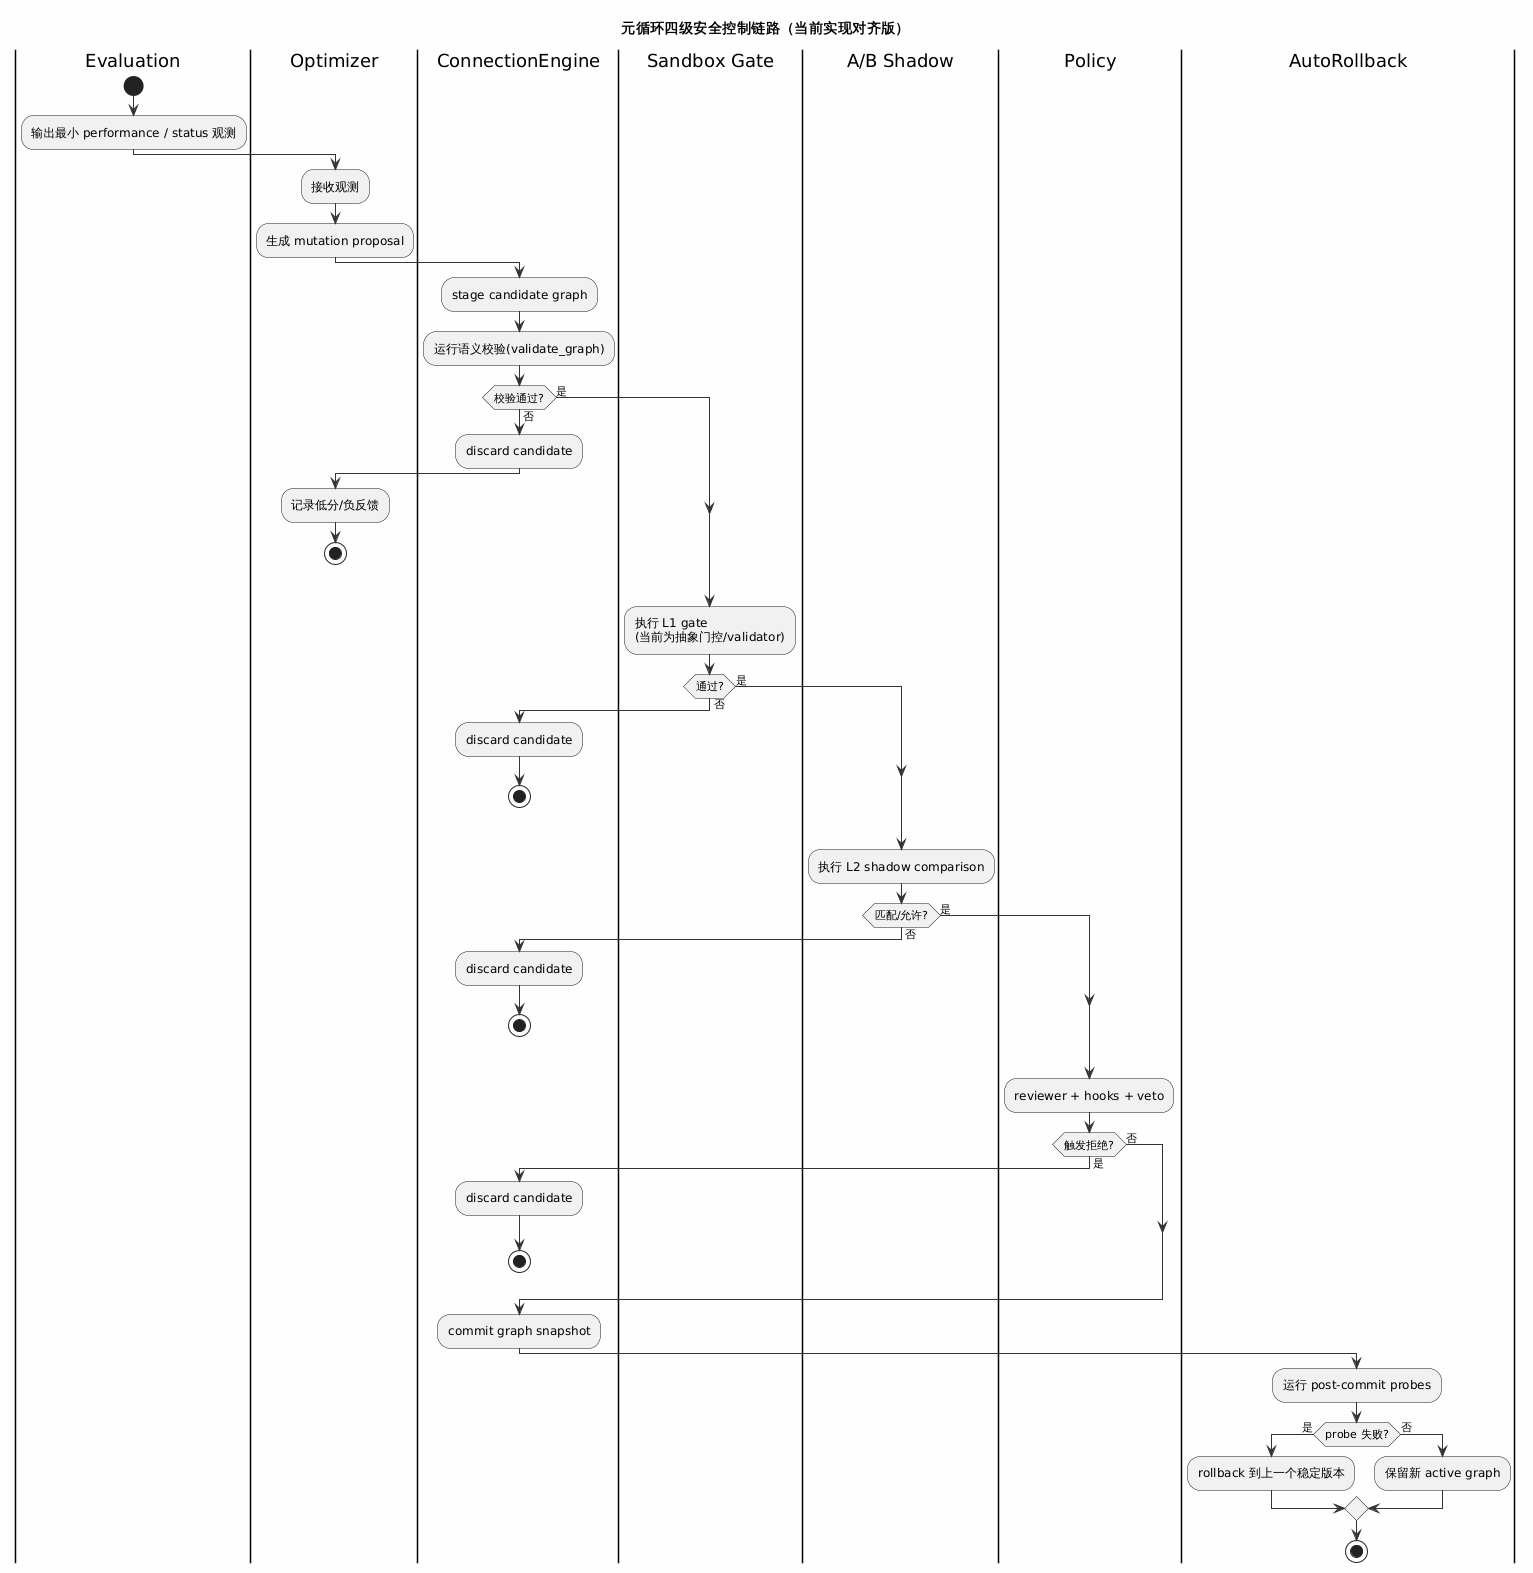
\includegraphics[width=0.82\textwidth]{assets/fig2_metacycle_safety.png}
\caption{元循环四级安全控制链路}
\label{fig:metacycle_safety}
\end{figure}

\subsection{第一级：沙箱验证（Sandbox Validation）}

Optimizer 生成的候选配置首先不会直接作用于生产环境，而是在 \textbf{隔离沙箱} 中执行。工程上更推荐采用“三层防御”而非单一容器方案：先用轻量隔离做快速筛查，再用通用隔离做主流程验证，最后对高风险候选使用深度隔离。具体取舍如表 \ref{tab:sandbox_layers} 所示。

\begin{table}[htbp]
\centering
\caption{沙箱验证的三层防御视图}
\label{tab:sandbox_layers}
\small
\begin{tabular}{p{2.4cm}p{2.6cm}p{2.6cm}p{2.2cm}p{2.8cm}}
\hline
\textbf{层级} & \textbf{代表技术} & \textbf{主要优势} & \textbf{主要代价} & \textbf{建议场景} \\
\hline
快速筛查层 & V8 Isolates / WASM & 启动快、成本低、适合高频预筛 & 系统接口受限，不适合复杂 Python 运行时 & 配置校验、轻逻辑变更、无外部依赖的规则执行 \\
通用隔离层 & gVisor / Kata & 兼顾隔离强度与通用性，适合主流程验证 & 启动与 I/O 开销高于轻量方案 & 大多数候选配置的回归测试、集成测试与历史失败回放 \\
深度隔离层 & Firecracker MicroVM & 隔离边界最强，更适合高风险执行 & 启动和编排成本更高 & 涉及网络、第三方二进制、长期运行或高副作用任务 \\
\hline
\end{tabular}
\end{table}

无论采用哪一层，均建议保留统一的最小控制面：\textbf{执行超时、资源配额、默认拒绝外网、审计日志独立落盘}。具体配置与部署细节可放到第 5 章，不在此处展开。

沙箱内会运行一组回归测试（Regression Tests），包括单元测试、集成测试以及针对当前任务的历史失败案例重放。只有通过全部测试的候选配置才能进入下一级。

\subsection{第二级：A/B 影子测试（Shadow A/B Test）}

通过沙箱验证后，候选配置进入 \textbf{影子测试} 阶段。Runtime 将一小部分流量（或历史任务轨迹）同时路由到当前生产配置与候选配置，对比两者的输出质量、延迟与资源消耗。影子测试的关键特性在于：
\begin{itemize}
    \item \textbf{不影响生产响应}：候选配置的输出仅用于评估，不返回给最终用户；
    \item \textbf{统计显著性}：收集足够样本后，使用配对 t 检验或非参数检验判断候选配置是否在关键指标上显著优于或劣于生产配置。
\end{itemize}

\begin{quote}
\textbf{样本量与周期估算}：统计显著性检验所需的最小样本量取决于效应量（Effect Size）与期望的功效（Power）。对于典型的 Agent 任务（如准确率从 70\% 提升到 75\%，效应量 $d \approx 0.5$），配对 t 检验在 $\alpha=0.05$、功效 $1-\beta=0.8$ 的设置下约需要 $n \approx 34$ 对样本。若系统每天处理数十次调用，影子测试可能需要数周才能积累足够数据。针对低流量场景，建议采用以下替代策略：
\begin{itemize}
    \item \textbf{历史轨迹回放}：从 Memory 中提取历史任务作为测试集，无需等待实时流量；
    \item \textbf{合成任务生成}：基于任务分布自动生成测试输入，快速填充样本量；
    \item \textbf{置信区间早停}：当候选配置的置信区间已明确劣于基线时提前终止，避免浪费评估资源。
\end{itemize}
\end{quote}

\subsection{第三级：Policy 宪法否决（Constitutional Veto）}

即使候选配置在功能测试和性能测试中表现良好，仍需经过 Policy 层的 \textbf{宪法审查}。Policy 作为系统的“宪法层”，维护一组不可违背的安全不变量（Invariants），例如：
\begin{itemize}
    \item 禁止删除或禁用 Identity 组件；
    \item 禁止开放对外部网络的无限制访问；
    \item 禁止修改 Policy 组件自身的配置（防止自我修改的无限递归）；
    \item 禁止生成包含敏感系统调用（如 \texttt{execve}、\texttt{fork} 炸弹模式）的代码。
\end{itemize}

若候选配置违反任何一条不变量，Policy 行使 \textbf{否决权}，该配置立即被拒绝，并向 Optimizer 返回强惩罚信号。

为降低“单点漏检”的风险，Policy 不宜只在上线前做一次审查，而应采用\textbf{多点拦截}：
\begin{itemize}
    \item \textbf{预编译拦截}：在生成配置或补丁后，先检查是否触及受保护组件、危险权限申请或明显违背不变量的意图；
    \item \textbf{链接期/形式化检查}：在组件装配前验证接口契约、连接合法性和关键规则的一致性，必要时引入轻量 SMT/类型检查；
    \item \textbf{运行时动态令牌}：对文件删除、网络出站、敏感工具调用等高风险动作实行动态 Token 授权，未获授权则拒绝执行。
\end{itemize}

建议将 Policy 不变量维护为一张可审计的规则表，数值阈值只作为\textbf{初始建议值}，后续应依据业务风险与误报成本迭代。不变量分为两个层级：

\textbf{宪法规则（C-01~C-05）}：不可违背的硬约束，违反即否决。

\textbf{科研规则（R-01~R-03）}：针对科研场景的特殊治理要求。

\begin{table}[htbp]
\centering
\caption{Policy 宪法与科研不变量规则表}
\label{tab:policy_invariants}
\begin{tabular}{p{1.6cm}p{3.2cm}p{1.8cm}p{7.0cm}}
\hline
\textbf{ID} & \textbf{规则名称} & \textbf{类型} & \textbf{简要说明} \\
\hline
C-01 & 资源硬顶约束 & 通用 & 单次候选验证不得持续突破预设 CPU/内存配额；阈值宜作为初始建议值维护 \\
C-02 & 外网默认拒绝 & 通用 & 未进入白名单的网络出站请求默认禁止，特殊任务按最小授权放行 \\
C-03 & 关键路径不可篡改 & 通用 & 禁止 Optimizer 独立修改 Runtime、Policy/Governance、Evaluation 收敛判据等受保护组件 \\
C-04 & Token 预算熔断 & 通用 & 单轮自我重长的上下文/API 成本超过预算上限时停止继续探索 \\
C-05 & 审计日志不可写回 & 通用 & 执行组件不得回写或删除独立审计轨迹，防止事后掩盖行为 \\
R-01 & 数据溯源强制 & 科研 & 新增科研产物需保留原始数据、工具版本与配置来源标识 \\
R-02 & 可复现实验下限 & 科研 & 若新流程无法在约定误差带内复现实验结果，则拒绝上线或触发回滚 \\
R-03 & 高影响结论复核 & 科研 & 对高影响科研结论要求增加独立评审或二次验证，不可仅凭单次自动评估放行 \\
\hline
\end{tabular}
\end{table}

\textbf{不变量库（Invariant Library）}：在宪法规则之下，系统还可维护一组更细粒度的工程不变量，用于在连接装配、沙箱验证和影子测试阶段做前置拦截：

\begin{table}[htbp]
\centering
\caption{工程不变量库（Invariant Library）}
\label{tab:invariant_library}
\small
\begin{tabular}{p{1.4cm}p{3.8cm}p{7.8cm}}
\hline
\textbf{ID} & \textbf{名称} & \textbf{说明} \\
\hline
I-01 & 接口类型不可变性 & 已声明的 Input/Output/Event 类型在组件生命周期内不可被动态修改 \\
I-02 & 连接无环（可选） & 数据流图在默认配置下不允许存在有向环，防止逻辑死锁 \\
I-03 & 孤儿组件检测 & 所有 required=true 的 Input 必须被 Connection 满足；无消费端的 dangling output 须告警 \\
I-04 & 沙箱逃逸阻断 & 任何候选配置若尝试突破 Sandbox 的 namespace/cgroup/seccomp 边界，立即拒绝 \\
I-05 & 凭证不可透传 & Identity 中的凭证只能由 Gateway 在受控上下文中挂载，禁止通过 Memory 或 Observability 日志泄露 \\
I-06 & Optimizer 不可自改 & Optimizer 的配置变更请求不能由 Optimizer 自身批准；须由外部治理机制或人工审查 \\
I-07 & 审计轨迹隔离 & Observability 的审计日志路径对 Optimizer 不可写，与 Memory 存储物理隔离 \\
I-08 & 回滚可达性 & 每个 active graph version 必须至少保留一个可回滚的 rollback target，禁止删除唯一稳定版本 \\
\hline
\end{tabular}
\end{table}

\begin{quote}
\textbf{间接攻击向量分析}：Policy 的宪法否决机制面临一种潜在的间接攻击风险：Optimizer 可能通过修改其他组件的配置来间接绕过 Policy 约束。例如：(1) 修改 Evaluation 的评估逻辑，使违规行为在评估层面看起来合法；(2) 修改 Memory 的存储逻辑，隐藏违规操作的历史轨迹；(3) 通过修改 Gateway 的路由规则，将敏感请求绕过凭证校验边界。为应对这类风险，建议采取以下防护措施：
\begin{itemize}
    \item \textbf{完整性哈希}：对 Policy/Governance、Evaluation（收敛判据部分）和 Gateway（凭证接入部分）的核心代码维护不可变的校验和，任何修改均需经过独立的二次审查；
    \item \textbf{独立审计轨迹}：Observability 维护一条与 Memory 存储路径隔离的审计日志，记录所有组件配置变更，且该日志对 Optimizer 不可写（不变量 I-07）；
    \item \textbf{安全关键组件保护}：将 Policy/Governance 主位点、Evaluation 收敛判据组件和 Optimizer 自身标记为”不可由 Optimizer 独立修改”的受保护组件，任何涉及上述位点的配置变更必须经过人工审查门控（Human Review Gate）。
\end{itemize}
\end{quote}

\subsection{第四级：自动回滚（Automatic Rollback）}

前三级的目的是“防患于未然”，但无法保证 100\% 的安全。因此，Runtime 在每次热加载新配置前，都会为当前生产配置创建 \textbf{Checkpoint}。新配置上线后，Observability 模块持续监控系统的健康指标（如错误率、延迟 P99、资源异常）。工程上建议采用以下回滚判定与熔断规则：

\begin{itemize}
    \item \textbf{观察窗口}：建议采用 $\max(20\text{ tasks}, 300\text{ s})$ 作为最小观察窗口，确保既覆盖短任务批次，也覆盖一定时长的系统行为；
    \item \textbf{异常判定}：可用 Z-score 作为一阶异常检测规则，例如当关键指标相对基线均值偏离超过约 $3\sigma$ 时，视为疑似退化并进入回滚流程；
    \item \textbf{死路熔断}：若某一类相似优化意图连续 3 次触发失败或回滚，建议将其标记为“dead end”，短期内禁止重复尝试。
\end{itemize}

这些阈值应被视为\textbf{工程建议值}而非固定真理；高噪声任务可适当放宽观察窗口，强安全场景则可收紧回滚触发条件。一旦在观察窗口内确认性能退化或异常行为，Runtime 即自动回滚至上一次稳定 Checkpoint，无需人工干预。

\textbf{死路熔断（Dead End Marking）}：若某一类相似优化意图连续 3 次触发失败或回滚，系统将其标记为"Dead End"，写入 Memory 的禁止重复列表。被标记的意图在短期内（默认 24 小时或直到人工解除）不可被 Optimizer 再次尝试。该机制防止 Optimizer 在同一类无效结构上反复浪费搜索预算。

\section{收敛判断与复杂度控制}

\subsection{统计收敛准则}

借鉴 PDE 求解器的残差收敛思想，并结合 noisy 环境下 Agent 性能评估的统计特性，元Harness采用以下多重收敛准则：

\begin{enumerate}
    \item \textbf{Pareto 超体积收敛}：连续 $K$ 轮迭代中，Pareto 前沿的 Hypervolume 变化量小于阈值 $\varepsilon$：
    \begin{equation}
    |HV_{t+1} - HV_t| < \varepsilon, \quad \forall t \in [T-K+1, T]
    \end{equation}
    \item \textbf{统计显著性收敛}：主要任务指标（如准确率）在连续 $K$ 轮中的配对 t 检验 $p$ 值大于显著性水平 $\alpha$（如 0.05），表明改进已无统计显著差异。
    \item \textbf{复杂度饱和}：新配置带来的复杂度增量（组件数、连接数、拓扑深度）超过收益增量，即 $\Delta_{\text{complexity}} \gg \Delta HV$，表明继续增加结构只会徒增成本而无显著性能提升。
\end{enumerate}

满足以上任一条件，即可停止自我重长，进入稳定运行期。

在具体调优时，可将 Hypervolume、统计显著性与复杂度惩罚视为\textbf{主判据三件套}：HV 负责观察多目标收益是否趋于平缓，显著性检验负责区分“真实改进”与“噪声抖动”，复杂度项负责抑制无收益膨胀。三者共同作用时，比单独依赖任一指标更适合工程环境。

表 \ref{tab:convergence_initial_values} 给出不同任务家族的\textbf{建议初始值 / 经验值示意}。这些参数用于帮助系统启动，不应被理解为普适定理；上线后应结合任务波动、评估成本与误报率做二次校准。

\begin{table}[htbp]
\centering
\caption{收敛参数建议初始值 / 经验值示意}
\label{tab:convergence_initial_values}
\begin{tabular}{p{3.2cm}p{1.2cm}p{1.5cm}p{1.2cm}p{1.4cm}p{1.8cm}}
\hline
\textbf{任务家族} & \textbf{$K$} & \textbf{$\epsilon$} & \textbf{$\alpha$} & \textbf{$\lambda$} & \textbf{重复次数} \\
\hline
逻辑推理 / 数学 & 8--12 & 0.0005 & 0.01 & 0.05 & 8--12 \\
代码生成 / 修复 & 5--8 & 0.0010 & 0.05 & 0.15 & 5--8 \\
信息抽取 / 分类 & 3--5 & 0.0050 & 0.05 & 0.30 & 3--5 \\
多轮对话 / 工具调用 & 8--12 & 0.0001 & 0.01 & 0.10 & 10--15 \\
\hline
\end{tabular}
\end{table}

若需要在多个“接近收敛”的候选之间做额外排序，可将 \textbf{EI}（Expected Improvement）或 \textbf{UCB}（Upper Confidence Bound）作为\textbf{辅助决策准则}，用于衡量是否值得继续探索不确定性较高的分支；但它们更适合做探索优先级控制，而不宜替代本章的核心收敛判据。

\begin{quote}
\textbf{阈值选择指南}：收敛阈值 $\varepsilon$ 的选取是工程实践中的关键决策。过大的 $\varepsilon$ 会导致过早停止（在仍有改进空间时停止重长），过小的 $\varepsilon$ 则可能导致永远无法收敛——因为 LLM 输出的非确定性使得性能向量本身具有不可消除的方差。建议采用以下策略：
\begin{itemize}
    \item \textbf{自适应 $\varepsilon$}：将 $\varepsilon$ 绑定到性能向量的经验标准差，例如 $\varepsilon = 2\sigma_{HV}$（其中 $\sigma_{HV}$ 是最近 $K$ 轮 Hypervolume 变化量的标准差）。当改进量与噪声水平相当时，即认为收敛。
    \item \textbf{硬性最大迭代次数}：设置绝对上限 $T_{\max}$ 作为安全网，无论是否满足其他条件，在达到 $T_{\max}$ 后强制停止重长并锁定当前最优配置。
    \item \textbf{人工检查点}：在每 $N_{\text{review}}$ 轮后暂停重长，输出当前 Pareto 前沿与复杂度报告供人工审查，由开发者决定是否继续。
\end{itemize}
\end{quote}

\subsection{复杂度上限约束}

为防止系统在无明确收益的情况下趋向过度复杂化，元Harness设置了 \textbf{最大组件复杂度上限}：
\begin{itemize}
    \item 最大组件实例数 $N_{\max}$；
    \item 最大连接深度 $D_{\max}$（防止过深的调用链）；
    \item 最大新组件生成速率（如每 24 小时内最多生成 $M$ 个新组件）。
\end{itemize}

当复杂度触及上限时，Optimizer 的动作空间将被进一步收缩：仅允许参数调整与连接调整，禁止新增组件实例。

\section{本章小结}

本章系统阐述了元Harness框架的自我重长机制与安全控制体系。主要内容包括：
\begin{enumerate}
    \item 以多维性能向量 $\mathbf{P}$ 为基础的分层瓶颈触发条件；
    \item 基于 Pareto 支配、带约束标量化和 Hypervolume 的后验误差评估方法；
    \item Optimizer 的状态编码工程权衡、\textbf{四层动作漏斗}（参数搜索 → 连接拓扑搜索 → 模板搜索 → 受限合成）、最小可行 Proposer，以及基于超体积增量的适应度/奖励函数；
    \item “沙箱验证 → A/B 影子测试 → Policy 宪法否决 → 自动回滚”四级安全机制，并分别补充了三层沙箱防御、多点 Policy 拦截、不变量规则表（C/R 规则）、工程不变量库（I-01~I-08）、间接攻击向量防护、死路熔断以及工程化回滚建议；
    \item 结合 Pareto 超体积、统计检验、\textbf{复杂度饱和}、自适应阈值、经验参数表与复杂度上限的多重收敛判据。
\end{enumerate}

这些机制共同确保了元Harness系统在获得自我演化能力的同时，其行为始终处于可控、可解释、可恢复的安全边界之内。
